%!TEX program = xelatex

\documentclass[compress]{beamer}
%--------------------------------------------------------------------------
% Common packages
%--------------------------------------------------------------------------
\usepackage[english]{babel}
\usepackage{pgfpages} % required for notes on second screen
\usepackage{graphicx}
\usepackage{subfigure}
\usepackage{multicol}
\usepackage{multirow}
\def\block(#1,#2)#3{\multicolumn{#2}{c}{\multirow{#1}{*}{$ #3 $}}}

\usepackage{fontspec}

\usepackage{tabularx,ragged2e}
\usepackage{booktabs}

\usepackage{setspace}

\usepackage{tcolorbox}
\usepackage{enumitem}
\usepackage{wrapfig}

%--------------------------------------------------------------------------
% Load theme
%--------------------------------------------------------------------------
\usetheme{hri}

\usepackage{dtklogos} % must be loaded after theme
\usepackage{tikz}
\usetikzlibrary{intersections,arrows,shapes,calc,mindmap,backgrounds,positioning,svg.path}

\graphicspath{{figs/}}

% to resize Blender's window:
% xdotool search --onlyvisible --classname "Blender" windowsize %@ 1032 709

\usepackage[cache]{minted}
\renewcommand{\theFancyVerbLine}{
  \sffamily\textcolor[rgb]{0.5,0.5,0.5}{\scriptsize\arabic{FancyVerbLine}}}

\newminted{glsl}{linenos=false,
                 fontsize=\tiny}


\tikzset{box/.style={
            draw, 
            orange,
            fill=blue!20,
            fill opacity=0.1,
            ultra thick,
            inner sep=0pt,
            minimum size=1cm,
            transform shape,
            rounded corners,
            anchor=north west
        },
        every edge/.style={
            draw,
            ultra thick,
            orange
        },
        textbox/.style={
            black,
            fill=white,
            fill opacity=0.8,
            text=black,
            text opacity=1,
            ultra thick,
            inner sep=10pt,
            minimum size=1cm,
            transform shape,
            rounded corners,
            font=\Medium
        }
}

\newcommand{\key}[1]{
    %\sffamily
    %\fcolorbox[RGB]{200,192,144}{200,248,200}{\textbf{#1}}
    %\normalfont

    \begin{tcolorbox}[tcbox raise=-1mm,center upper,colback=yellow!20!white,top=1.3pt,right=3pt,left=3pt,boxsep=0pt,boxrule=0.4pt,hbox,height=5mm,bottomrule=1mm]%
        {\normalsize \sc #1}%
    \end{tcolorbox}
}

\newcommand{\rmb}{
\includegraphics[height=1.5em]{RMB}~}
\newcommand{\lmb}{
\includegraphics[height=1.5em]{LMB}~}
\newcommand{\mmb}{
\includegraphics[height=1.5em]{MMB}~}

\newcommand{\omode}{
\includegraphics[height=1.5em]{object_mode}~}
\newcommand{\emode}{
\includegraphics[height=1.5em]{edit_mode}~}
\newcommand{\smode}{
\includegraphics[height=1.5em]{sculpt_mode}~}
\newcommand{\tmode}{
\includegraphics[height=1.5em]{texpaint_mode}~}

\newcommand{\imageicon}{
\includegraphics[height=1.5em]{image_icon}~}

%--------------------------------------------------------------------------
% General presentation settings
%--------------------------------------------------------------------------
\title{Modelisation 3D avec Blender}
\subtitle{CS211 -- Introduction à l'informatique visuelle}
\date{31 mars 2015}
\author{Séverin Lemaignan}
\institute{Computer-Human Interaction\\for Learning and Instruction {\Medium
EPFL}}

%--------------------------------------------------------------------------
% Notes settings
%--------------------------------------------------------------------------
%\setbeameroption{show notes on second screen}
%\setbeameroption{hide notes}

\begin{document}

\maketitle

\begin{frame}{}
    Lorenzo Lucignano:
    \begin{quote}\Medium
        ``Even Satan wouldn't have came up with the Blender UI!''
    \end{quote}
\end{frame}

\imageframe{lorenzo}


\bgframe[blender1.png]{

    
\begin{tikzpicture}[remember picture,overlay]

        \only<1>{
            \node[box] (zone1) at (1,3.1) [minimum width=5.2cm,minimum height=7.1cm] {};
            \node[textbox] at (8,0) {3D viewport} edge (zone1);
        }
        \only<2>{
            \node[box] (zone1) at (-1,3.1) [minimum width=2.2cm,minimum height=7.1cm] {};
            \node[textbox] at (5,0) {Toolshelf (\key{T} to toggle)} edge (zone1);
        }
        \only<3>{
            \node[box] (zone1) at (6.2,3.1) [minimum width=2.2cm,minimum height=7.1cm] {};
            \node[textbox] at (2,0) {Properties panel (\key{N} to toggle)} edge (zone1);
        }
        \only<4>{
            \node[box] (zone1) at (8.3,3.1) [minimum width=3.4cm,minimum height=1.4cm] {};
            \node[textbox] at (7,0) {Outliner} edge (zone1);
        }

        \only<5>{
            \node[box] (zone1) at (8.3,1.8) [minimum width=3.4cm,minimum height=7.2cm] {};
            \node[textbox] at (3,0) {Properties} edge (zone1);
        }
    \end{tikzpicture}
}

\bgframe[blender1.png]{

    \begin{tikzpicture}[remember picture,overlay]
            \node[box] (zone1) at (8.1,3.15) [minimum width=0.4cm,minimum height=0.4cm] {};
            \node[box] (zone2) at (8.1,-4.2) [minimum width=0.4cm,minimum height=0.4cm] {};
            \node[box] (zone3) at (8.25,1.95) [minimum width=0.4cm,minimum height=0.4cm] {};
            \node[textbox] at (5,0) {Split/joint areas} edge (zone1) edge (zone2) edge (zone3);
    \end{tikzpicture}
}


\bgframe[blender2.png]{

    \begin{tikzpicture}[remember picture,overlay]
        \only<1>{
            \node[box] (zone1) at (-0.85,1.8) [minimum width=2.1cm,minimum height=6.1cm] {};
            \node[textbox] at (5,0) {Select the window's type} edge (zone1);
        }
    \end{tikzpicture}
}

\bgframe[blender3.png]{

    \begin{tikzpicture}[remember picture,overlay]
        \only<1>{
            %\grid
            \node[box] (zone1) at (1.9,-2.2) [minimum width=1.65cm,minimum height=2cm] {};
            \node[textbox] at (5,0) {Select the mode} edge (zone1);
        }
    \end{tikzpicture}
}


\bgframe[blender4.png]{

    \begin{tikzpicture}[remember picture,overlay]
        \only<1>{
            %\grid
            \node[box] (zone1) at (8.5,-0.5) [minimum width=3.2cm,minimum height=1.4cm] {};
            \node[box] (zone2) at (9.5,1.65) [minimum width=0.4cm,minimum height=0.4cm] {};
            \node[textbox] at (5,0) {Set the units} edge (zone1) edge (zone2);
        }
    \end{tikzpicture}
}

\renewcommand{\key}[1]{
    \fcolorbox{black}{yellow!20!white}{#1}
}


\begin{frame}{Blender Cheat Sheet}
    \tiny
    \begin{multicols}{2}
        {\Medium In the 3D viewport}
        \begin{itemize}[leftmargin=0.1cm]
            \item \lmb to move the 3D cursor, \rmb to select
            \item \mmb to rotate, \key{shift} + \mmb to pan
            \item \key{space} to search for an action/operator
            \item \key{shift+A} to add an object
            \item \key{tab} to switch between Edit mode and Object mode
            \item \key{Z} to switch between wireframe and solid rendering
            \item \key{G}\key{R}\key{S} to move ({\Medium g}o to), {\Medium r}otate, {\Medium s}cale objects
            \item \key{X}\key{Y}\key{Z} to constraint along one axis (twice: local axes) 
            \item type any numerical value to manually set the translation/rotation/scale
            \item \key{E} to {\Medium e}xtrude selected face or edge
        \end{itemize}

        {\Medium Selection}
        \begin{itemize}[leftmargin=0.1cm]
            \item \rmb to select
            \item \key{A}: (de)select {\Medium a}ll
            \item \key{B}: rectangular ({\Medium b}ox) selection
            \item \key{C} + \lmb: interactive selection (\rmb when done)
        \end{itemize}
    \end{multicols}

\end{frame}

\imageframe{final-render}


\begin{frame}{Étape 1 : modélisation}
        \centering
        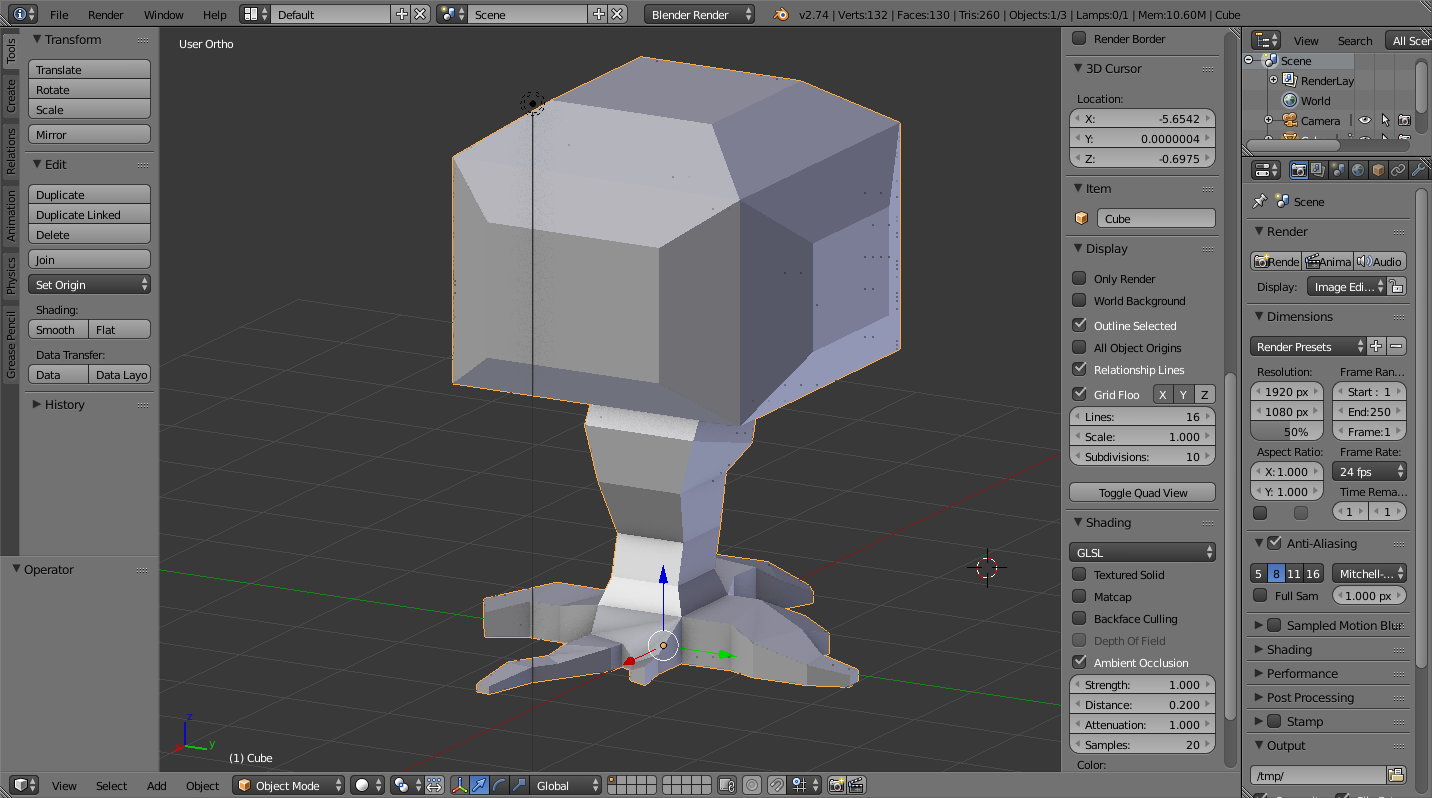
\includegraphics[width=0.9\linewidth]{tree1.png}
\end{frame}

%\videoframe{jingle.ogg}

\begin{frame}{Étape 2 : matériaux de base}
        \centering
        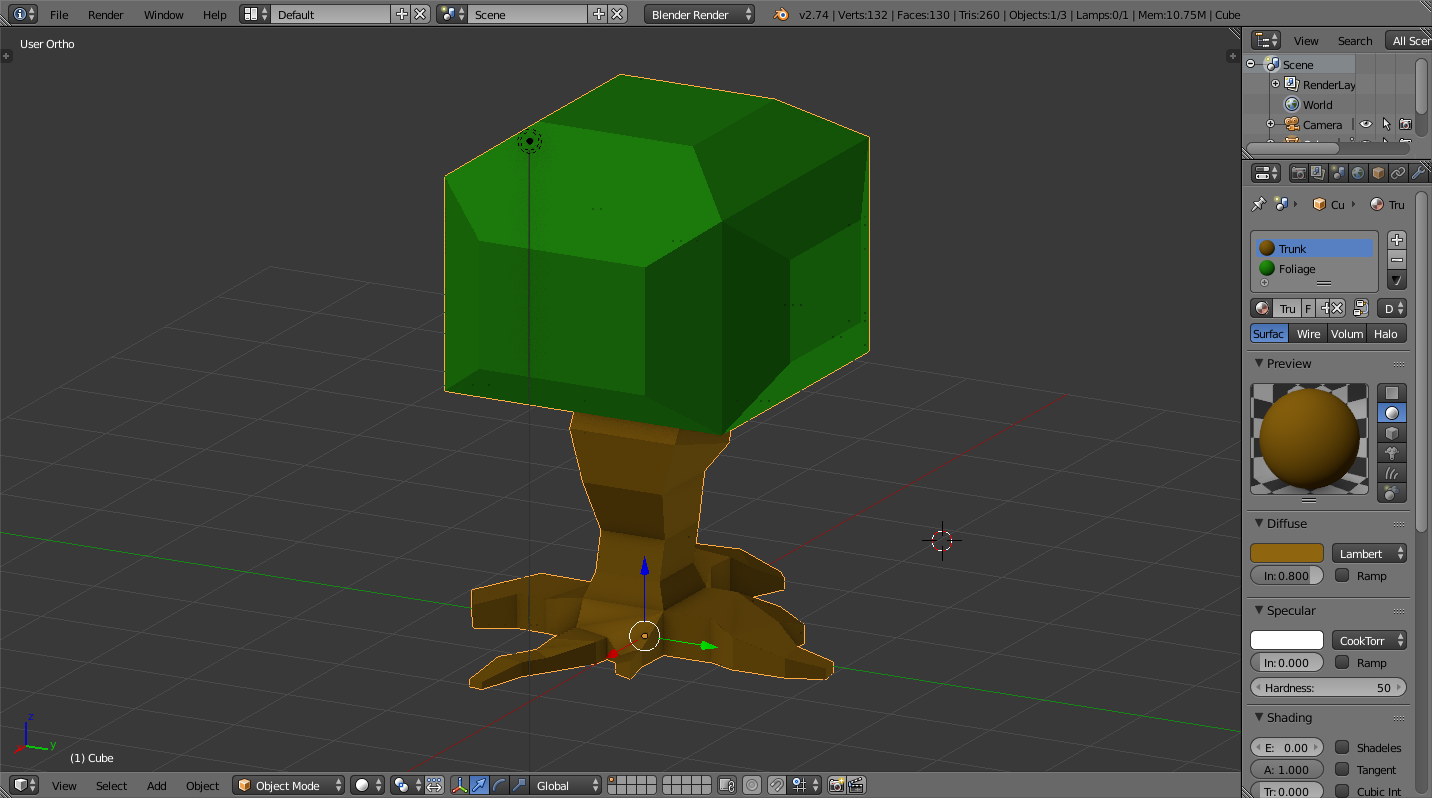
\includegraphics[width=0.9\linewidth]{tree2.png}
\end{frame}

%\videoframe{jingle.ogg}


\begin{frame}{Étape 3 : la sculpture 3D}
        \centering
        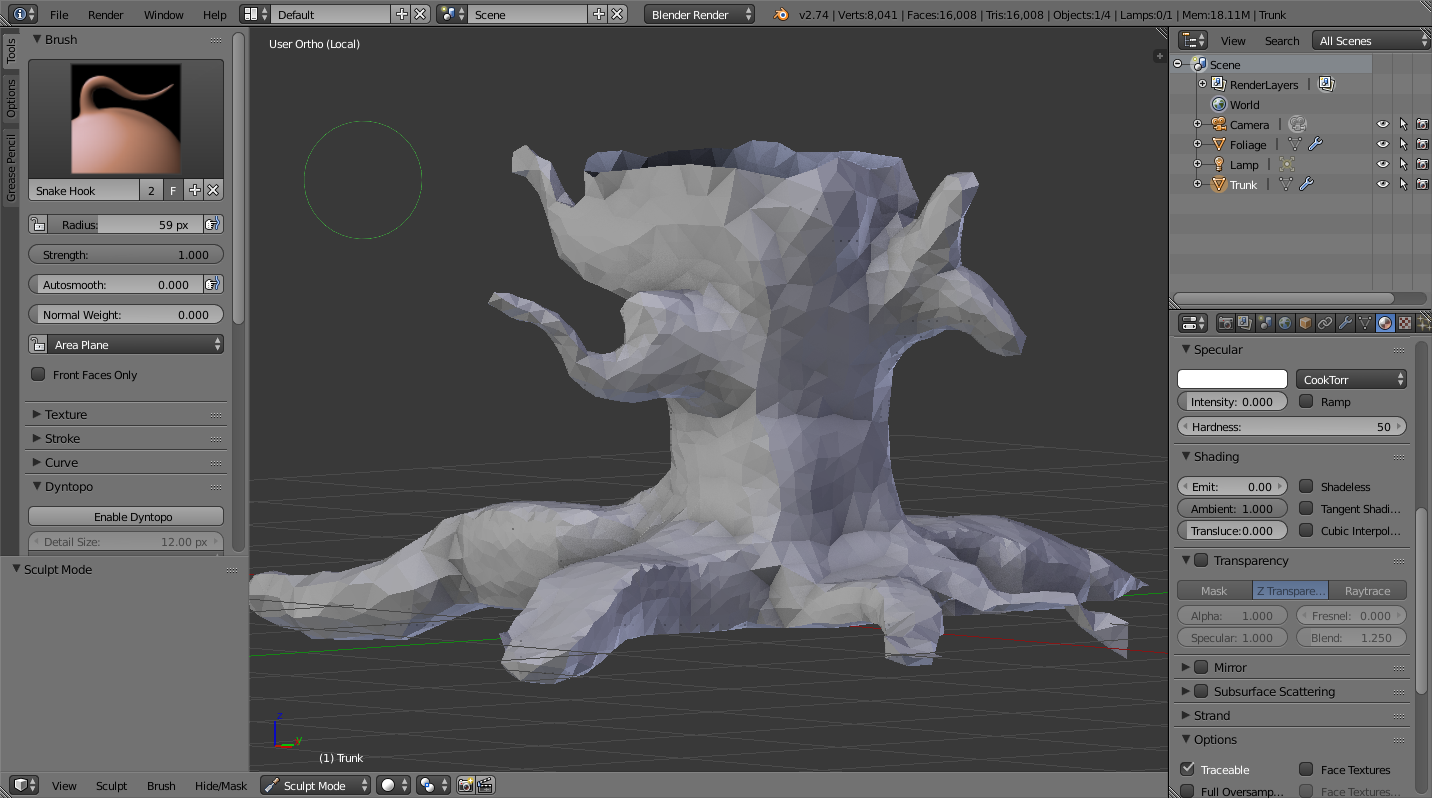
\includegraphics[width=0.9\linewidth]{tree4.png}
\end{frame}

%\videoframe{jingle.ogg}


\begin{frame}{Étape 4 : peindre les textures}
        \centering
        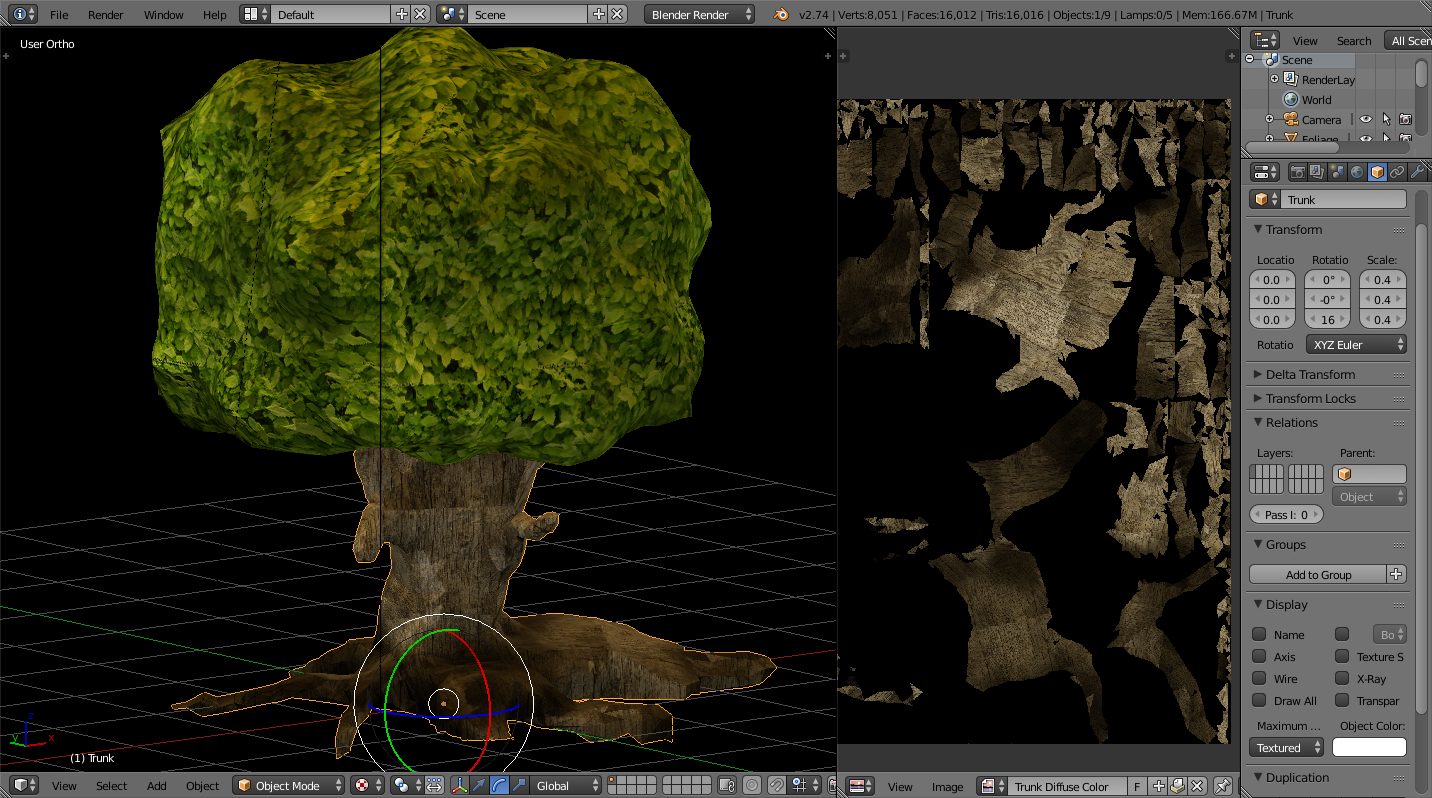
\includegraphics[width=0.9\linewidth]{tree5-2.png}
\end{frame}

\begin{frame}{Les étapes pour peindre les textures (1)}
    \tiny
    \begin{multicols}{2}
        Créez tout d'abord une nouvelle fênetre de type {\Medium UV/Image Editor}:\\
        \begin{center}
        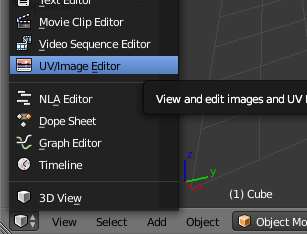
\includegraphics[width=2cm]{uv-image-window}
        \end{center}

        1- {\Medium Unwraping} de l'objet en {\Medium Edit Mode \emode}
        \begin{itemize}[leftmargin=0.1cm]
            \item sélectionner toutes les faces \key{A}
            \item \key{U} puis {\Medium Smart UV Project} : le UV map devrait s'afficher dans le UV Editor.
        \end{itemize}

        2- Peinture de la texture en mode {\Medium Texture Paint \tmode}
        \begin{itemize}[leftmargin=0.1cm]
            \item (si le Toolshelf n'est pas affiché, affichez-le \key{T})
            \item Créez une texture vide (noire) en cliquant sur {\Medium Add
                Paint Slot} and le Toolshelf, puis {\Medium Diffuse Color}, puis
                {\Medium Ok}. Votre objet devrait maintenant être noir.  Vous
                pouvez commencer à le peindre (\lmb).
            \item Dans la fenêtre {\Medium UV/Image Editor}, cliquez sur
                \imageicon et choississez la texture que vous venez de créer :
                vous la verrez se mettre à jour automatiquement pendant que vous
                peignez.
            \item {\Medium Important !} Les textures ne sont pas sauvegardées
                automatiquement avec le {\tt .blend} ! Sauvegardez-les régulièrement
                via {\Medium Image>Pack as Image}.

        \end{itemize}
    \end{multicols}

\end{frame}

\begin{frame}{Les étapes pour peindre les textures (2)}
    \tiny
    \begin{multicols}{2}
        3- Peindre avec une texture

        \begin{itemize}[leftmargin=0.1cm]
            \item Dans le Toolshelf, cliquez sur {\Medium Texture} puis {\Medium
                New}.  Ceci crée une nouvelle texture (pour l'instant
                complètement noire), nommée {\tt Texture} par défaut.


            \item Ouvrez le panneau {\Medium Texture} de la fênetre {\Medium
                Properties} de votre objet, sélectionnez le premier slot {\tt Tex}
                et remplacez-le par la texture {\tt Texture}:
                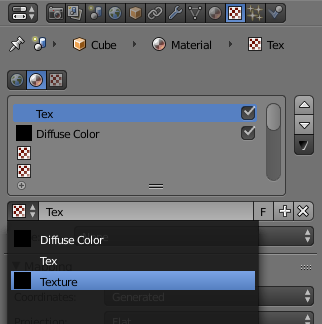
\includegraphics[width=2cm]{texture1}

            \item Cliquez sur {\Medium Open} pour ouvrir une image.
            
            \item Vous pouvez maintenant peindre votre objet avec cette texture.

        \end{itemize}

    \end{multicols}

\end{frame}



%\videoframe{jingle.ogg}

\begin{frame}{Étape 5 : l'illumination}
        \centering
        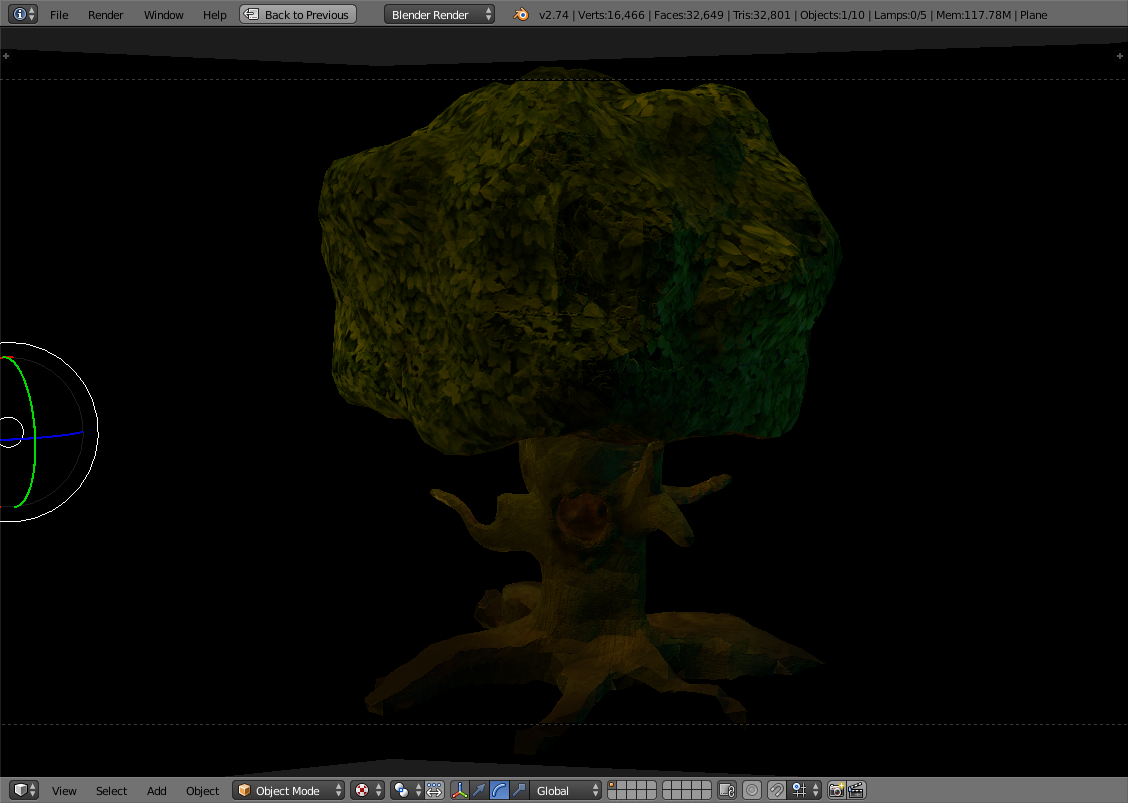
\includegraphics[width=0.9\linewidth]{tree6.png}
\end{frame}

%\videoframe{jingle.ogg}

\begin{frame}{Tâche 1: Avec les Lego...}
         \centering
        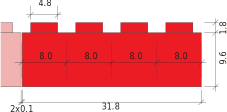
\includegraphics[width=0.9\linewidth]{lego}
\end{frame}

\begin{frame}{Tâche 1: Array modifier!}
         \centering
        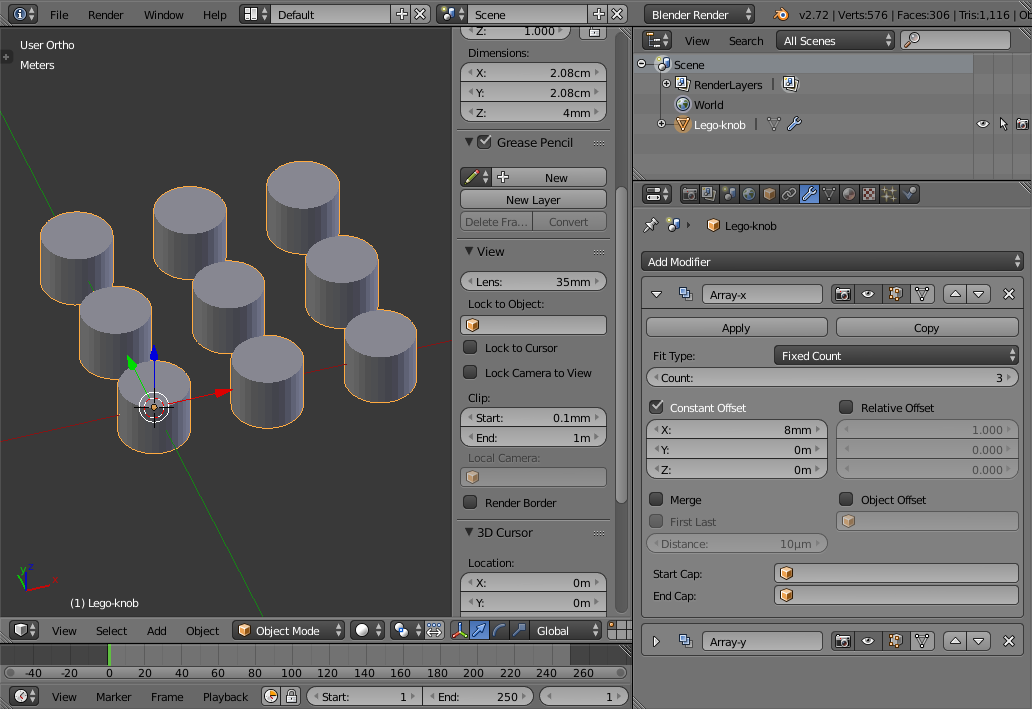
\includegraphics[width=0.9\linewidth]{array}
\end{frame}

\begin{frame}{Tâche 1: Boolean modifier!}
         \centering
        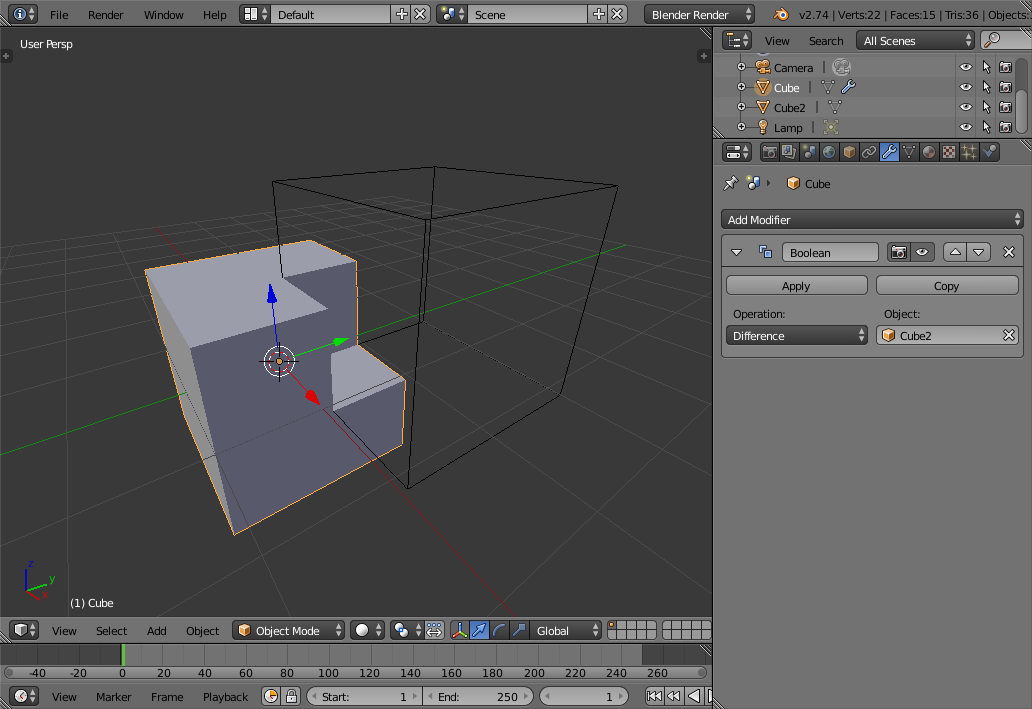
\includegraphics[width=0.9\linewidth]{boolean}
\end{frame}



\begin{frame}{Tâche 2: L'environnement du jeu}
         \centering
        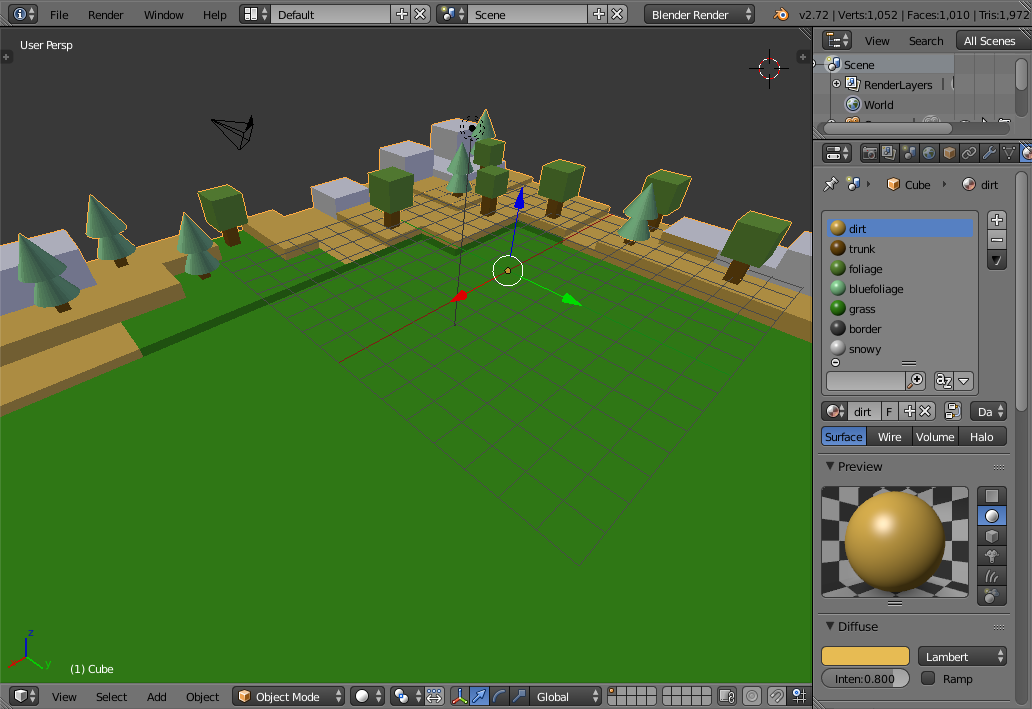
\includegraphics[width=0.9\linewidth]{env}
\end{frame}


\begin{frame}{}
    \begin{center}
        \Large
        That's all, folk!\\[2em]
        \normalsize
        Questions : \url{severin.lemaignan@epfl.ch} \\
        %Slides : \url{github.com/severin-lemaignan/intro-3d-computer-graphics}
    \end{center}
\end{frame}
\end{document}






